% Created 2021-07-16 Fri 18:51
% Intended LaTeX compiler: pdflatex
\documentclass[11pt]{article}
\usepackage[utf8]{inputenc}
\usepackage[T1]{fontenc}
\usepackage{graphicx}
\usepackage{grffile}
\usepackage{longtable}
\usepackage{wrapfig}
\usepackage{rotating}
\usepackage[normalem]{ulem}
\usepackage{amsmath}
\usepackage{textcomp}
\usepackage{amssymb}
\usepackage{capt-of}
\usepackage{hyperref}
\usepackage{chemfig}
\usepackage{mhchem}
\author{Shaurya Singh}
\date{\today}
\title{Ap Chem Summer Assignment \#1}
\hypersetup{
 pdfauthor={Shaurya Singh},
 pdftitle={Ap Chem Summer Assignment \#1},
 pdfkeywords={},
 pdfsubject={},
 pdfcreator={Emacs 28.0.50 (Org mode 9.5)}, 
 pdflang={English}}
\begin{document}

\maketitle

\section{Summer Assignment 1}
\label{sec:orgca3dbeb}
\subsection{How many significant figures are there each of the following values}
\label{sec:org354d6b2}
\begin{enumerate}
\item \(0.002330\) has \textbf{4} significant figures. Since the leading zeroes (those before the 2) don't count, the significant figures consist of \(2330\), or 4 significant figures.
\item \(13.00\) has \textbf{4} significant figures. Since all non-zero digits are significant (the 13) as well as all digits after the decimal, every digit in this number is significant, giving us 4 significant figures.
\item \(322.1221\) has \textbf{7} significant figures. Since all non-zero digits are significant, every digit in this number is significant. That gives us 7 significant figures.
\item \(1204.30\) has \textbf{6} significant figures. Since all non-zero digits are significant (the 12 4.3) as well as all digits after the decimal and zeroes between non-zero digits, every digit in this number is significant, giving us 6 significant figures.
\item \(0.0002\) has \textbf{1} significant figure. Since all leading zeroes (those before the 2) don't count, the significant figures consist of just the 2, which means it has only 1 significant figure.
\item \(2200.0\) has \textbf{5} significant figures. Since all non-zero digits (the 22) as well as zeroes before and after the decimal point are sig figs, all 5 digits are significant figures.
\item \(0.0331120\) has \textbf{6} significant figures. Since all non-zero digits (33112) as well as the zeroes after the non-zero digits are significant figures, there are 6 significant figures.
\end{enumerate}

\subsection{Perform the indicated calculations on the following measured values, giving the final answer with the correct number of significant figures.}
\label{sec:orgcff167b}
\begin{enumerate}
\item \(16.81 + 3.2257 = 20.0357 \approx 20.04\)
\item \(324.6 * 815.991 = 264870.6786 \approx 264900\)
\item \(2.85 + 3.4621 + 1.3 = 7.6121 \approx 7.6\)
\item \(7.442 - 7.429 = 0.013\)
\item \(1.65 * 14 = 23.1 \approx 23\)
\item \(\frac{27}{4.148} = 6.509161 \approx 6.5\)
\item \([\frac{(3.901 - 3.887)}{3.901}] * 1.00 = [\frac{0.014}{3.901}] * 1.00 \approx 0.0036 * 1.00 = 0.0036\)
\item \(6.404 * 2.91 * (18.7 - 17.1) = 6.404 * 2.91 * 1.6 \approx 30\)
\end{enumerate}

\subsection{A sample of motor oil with a mass of 440 g occupies 500 mL. What is the density of the motor oil?}
\label{sec:orgd660ba5}
We have the following values:
\begin{align*}
&d = ?\\
&m = 440g\\
&v = 500mL
\end{align*}
We can utilize the formula \(d=\frac{m}{v}\) (density = mass/volume)
\begin{align*}
d&=\frac{m}{v}\\
&=\frac{440g}{500mL}\\
&=0.88\frac{g}{mL}\\
&\approx0.9\frac{g}{mL}
\end{align*}
Therefore the density of the motor oil is \(\approx0.9\frac{g}{mL}\)

\subsection{The density of an object is 16.3 g/mL. Its volume is 0.125 L. What is the mass of the object?}
\label{sec:orgc60a873}
We can apply vector analysis to solve for the correct units
\begin{center}
\begin{tabular}{ll}
16.3g & 1000 mL\\
\hline
1mL & 1L\\
\end{tabular}
\end{center}
We are left with
\begin{align*}
&= \frac{16.3g * 1000mL}{(mL)(L)}\\
&= \frac{16.3g * 1000\xout{mL}}{\xout{(mL)}(L)}\\
&= \frac{16300g}{(L)}\\
&= 16300g/L
\end{align*}
Now we have the following values:
\begin{align*}
&d = 16300g/L\\
&m = \ ?\\
&v = 0.125L
\end{align*}
We can plug these variables into \(d=\frac{m}{v}\) to calculate for mass
\begin{align*}
16300{g}/{L} &=\frac{m}{0.125L}\\
\end{align*}
Re-arranging the equation in terms of mass, we get the following
\begin{align*}
m &= 16300 * 0.125\ \frac{g\xout{L}}{\xout{L}}\\
&= 2037.5g\\
&\approx 2040g
\end{align*}
The mass of the object is \(\approx 2040g\)

\subsection{A sample of uranium weighing 30.923 g was dropped in a graduated cylinder containing 22.30 mL of water. The volume of the water plus the sample was 23.90 mL. What is the density of uranium?}
\label{sec:org12fd442}
The volume of the object is going to be the difference between the volume of the water and the volume of the water + object.
\begin{equation}
23.90mL - 22.30mL = 1.60mL
\end{equation}
Now we have the following values:
\begin{align*}
&d = ?\\
&m = 30.923g\\
&v = 1.60mL
\end{align*}
We can apply the same \(d=\frac{m}{v}\) to calculate for density
\begin{align*}
d&=\frac{m}{v} \\
            &=\frac{30.923g}{1.60mL}\\
            &=19.33\frac{g}{mL}\\
            &\approx19.3\frac{g}{mL}
\end{align*}
Uranium has a density of \(\approx19.3\frac{g}{mL}\)

\subsection{How many protons, neutrons and electrons are in each of the following ions?}
\label{sec:org5d1a273}
\begin{enumerate}
\item The ion will have \textbf{26 protons}, since the atomic number is 26. It will also have \textbf{30 neutrons} since the mass \# is 56, and \(56-26=30\). Since it has a 3+ charge, there will be 3 more protons than electrons. \(26-3=23\), giving us \textbf{23 electrons}.
\item The ion will have \textbf{20 protons}, since the atomic number is 20. It will also have \textbf{20 neutrons} since the mass \# is 40, and \(40-20 = 20\). Since the charge is 2+, there will be 2 more protons than electrons, and \(20-2=18\), giving us \textbf{18 electrons}
\item The ion will have \textbf{9 protons}, since the atomic number is 9. It will also have \textbf{10 neutrons} since the mass \# is 19, and \(18-9=10\). Since the charge is 1-, there will be one more electron than proton. \(9+1=10\), giving us \textbf{10 electrons}
\item The ion will have \textbf{15 protons} since the atomic number is 15. It will also have \textbf{16 neutrons}, since the mass \# is 31, and \(31-15=16\). Since the charge is 3-, there will be 3 more electrons than protons. \(15+3=18\), giving us \textbf{18 electrons}
\item The ion will have \textbf{53 protons}, since the atomic number is 53. It will also have \textbf{74 neutrons}, since the mass \# is 127, and \(127-53=74\). Since the charge is 1-, there will be 1 more electron than protons. \(53+1=54\), giving us \textbf{54 electrons}.
\item The ion will have \textbf{53 protons}, since the atomic number is 53. It will also have \textbf{74 neutrons}, since the mass \# is 127, and \(127-53=74\). Since the charge is 7+, there will be 7 more protons than electrons. \(53-7=46\), giving us \textbf{46 electrons}.
\end{enumerate}

\subsection{Given the position in the periodic table, what is the most likely oxidation state (or common ion charge) that each element will have when forming an ion?}
\label{sec:org5a49496}
\begin{enumerate}
\item \(\ce{Cs}\) has a 1+ oxidation state
\item \(\ce{N}\) has a 3- oxidation state
\item \(\ce{Br}\) has a 1- oxidation state
\item \(\ce{K}\) has a 1+ oxidation state
\item \(\ce{Al}\) has a 3+ oxidation state
\item \(\ce{S}\) has a 2- oxidation state
\end{enumerate}

\subsection{Would you expect the following atoms to gain or lose electrons when forming an ion? If so, how many would be gained or lost?}
\label{sec:orgf28d06e}
\begin{enumerate}
\item \(\ce{Be}\) is in Group 2, therefore it will lose 2 electrons
\item \(\ce{Cl}\) is in Group 17, therefore it will gain 1 electron
\item \(\ce{Al}\) is in Group 13, therefore it will lose 3 electrons
\item \(\ce{O}\) is in Group 16, therefore it will gain 2 electrons
\item \(\ce{F}\) is in Group 17, therefore it will gain 1 electron
\item \(\ce{Li}\) is in Group 1, therefore it will lose 1 electron
\end{enumerate}

\subsection{Name each of the following compounds:}
\label{sec:org296ce5f}
\begin{enumerate}
\item \(\ce{PbI2}\) is named as Lead(II) iodide
\item \(\ce{NH4Cl}\) is named as Ammonium chloride
\item \(\ce{Fe2O3}\) is named as Iron(III) oxide
\item \(\ce{LiH}\) is named as Lithium hydride
\item \(\ce{CsCl}\) is named as Cesium chloride
\item \(\ce{Cr(OH)1}\) is named as Chromium(III) hydroxide
\item \(\ce{NaC2H2O2}\) is named as Sodium acetate
\item \(\ce{K2Cr2O7}\) is named as Potassium dichromate
\item \(\ce{Na2SO4}\) is named as Sodium sulfate
\end{enumerate}

\subsection{Which of the following particulate diagrams best shows the formation of water vapor from hydrogen gas and oxygen gas in a rigid container at 125\textdegree{} C?}
\label{sec:org9856277}
The correct answer would be \textbf{C}. Both Oxygen and Hydrogen exist freely as molecules with two atoms each, which eliminates options A and B. As the chemical composition of water is \(\ce{H2O}\), there need to be twice as many hydrogen molecules as oxygen molecules, and so C is the only answer that makes sense.

\subsection{Name each of the following compounds. In addition, for the compounds in letters a-c, draw Lewis structures, predict VSEPR geometry and hybridization.}
\label{sec:org58b7961}
\(\ce{NI3}\) is named as Nitrogen triiodide, and has the following Lewis Structure. It has a Trigonal pyramidal shape with 109.5° bond angles, and has a SP3 hybridization
\begin{align}
\chemfig{\charge{90=\:}{N}(-\charge{90=\:, 0:2pt=\:, -90=\:}{I})(-[:-90]\charge{0:2pt=\:, -90=\:, -180:2pt=\:}{I})(-[:-180]\charge{90=\:, -180:2pt=\:, -90=\:}{I})}
\end{align}
\(\ce{NH3}\) is named as Ammonia, and has the following Lewis Structure. It has a trigonal pyramid shape with 107° bond angles, and has a SP3 hybridization
\begin{align}
\chemfig{\charge{90=\:}{N}(-{H})(-[:-90]{H})(-[:-180]{H})}
\end{align}
\(\ce{CO}\) is named as Carbon monoxide, and has the following Lewis Structure. It has a linear shape with 180\textdegree{} Bond angles, and has a SP hybridization
\begin{align}
\chemfig{\charge{180=\:}{C}(~\charge{0=\:}{O})}
\end{align}
\begin{itemize}
\item \(\ce{P4O10}\) is named as tetraphosphorus decaoxide,
\item \(\ce{N2O4}\) is named as Dinitrogen tetroxide,
\item \(\ce{PCl3}\) is named as Phosphorus trichloride
\end{itemize}

\subsection{Molecules that have geometries in one plane include which of the following? Draw the Lewis structures to prove your point}
\label{sec:org5b1e616}
The lewis structure for \(\ce{BCl3}\)
\begin{center}
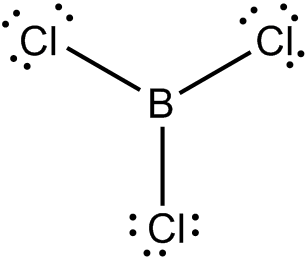
\includegraphics[width=75px]{/Users/shauryasingh/Documents/notes/class/orgs/chem/images/BCL3.png}
\end{center}
The lewis structure for \(\ce{CHCl3}\) is
\begin{align}
\chemfig{{C}(-\charge{90=\:, 0:2pt=\:, -90=\:}{Cl})(-[:-90]\charge{0:2pt=\:, -90=\:, -180:2pt=\:}{Cl})(-[:-180]\charge{90=\:, -180:2pt=\:, -90=\:}{Cl})(-[:-270]{H})}
\end{align}
The lewis structure for \(\ce{NCl3}\) is
\begin{align}
\chemfig{\charge{90=\:}{N}(-\charge{90=\:, 0:2pt=\:, -90=\:}{Cl})(-[:-90]\charge{0:2pt=\:, -90=\:, -180:2pt=\:}{Cl})(-[:-180]\charge{90=\:, -180:2pt=\:, -90=\:}{Cl})}
\end{align}
Therefore, the correct option is \textbf{A}. Both options II and III are tetrahedral and trigonal pyramidal respectively. Option I (\(\ce{BCL3}\)) is the only one that has a geometry in one plane (trigonal planar)

\subsection{The electron-dot structure (Lewis structure) for which of the following molecules would have two lone pairs of electrons on the central atom? Again, draw the Lewis structures to prove your point.}
\label{sec:orge19c437}
The lewis structure for \(\ce{H2S}\) is
\begin{center}
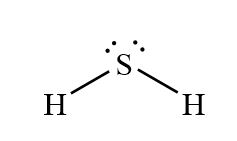
\includegraphics[width=75px]{/Users/shauryasingh/Documents/notes/class/orgs/chem/images/H2S.png}
\end{center}
The lewis structure for \(\ce{NH3}\) is
\begin{align}
\chemfig{\charge{90=\:}{N}(-{H})(-[:-90]{H})(-[:-180]{H})}
\end{align}
The lewis structure for \(\ce{CH4}\) is
\begin{align}
\chemfig{{C}(-{H})(-[:-90]{H})(-[:-180]{H})(-[:-270]{H})}
\end{align}
The lewis structure for \(\ce{HCN}\) is
\begin{align}
\chemfig{{H}-{C}(~\charge{0=\:}{N})}
\end{align}
The lewis structure for \(\ce{CO2}\) is
\begin{align}
\chemfig{(\charge{90=\:,-90=\:}{O})={C}=(\charge{90=\:,-90=\:}{O})}
\end{align}
Therefore, the only correct answer is \(\ce{H2S}\)

\subsection{Draw Lewis structures for (a) C2H2, (b) H2O, (c) NH3, (d) HCl (e) CCl4}
\label{sec:orgad49abf}
The lewis structure for \(\ce{C2H2}\) is
\begin{align}
\chemfig{{H}-{C}~{C}-{H}}
\end{align}
The lewis structure for \(\ce{H2O}\) is
\begin{center}
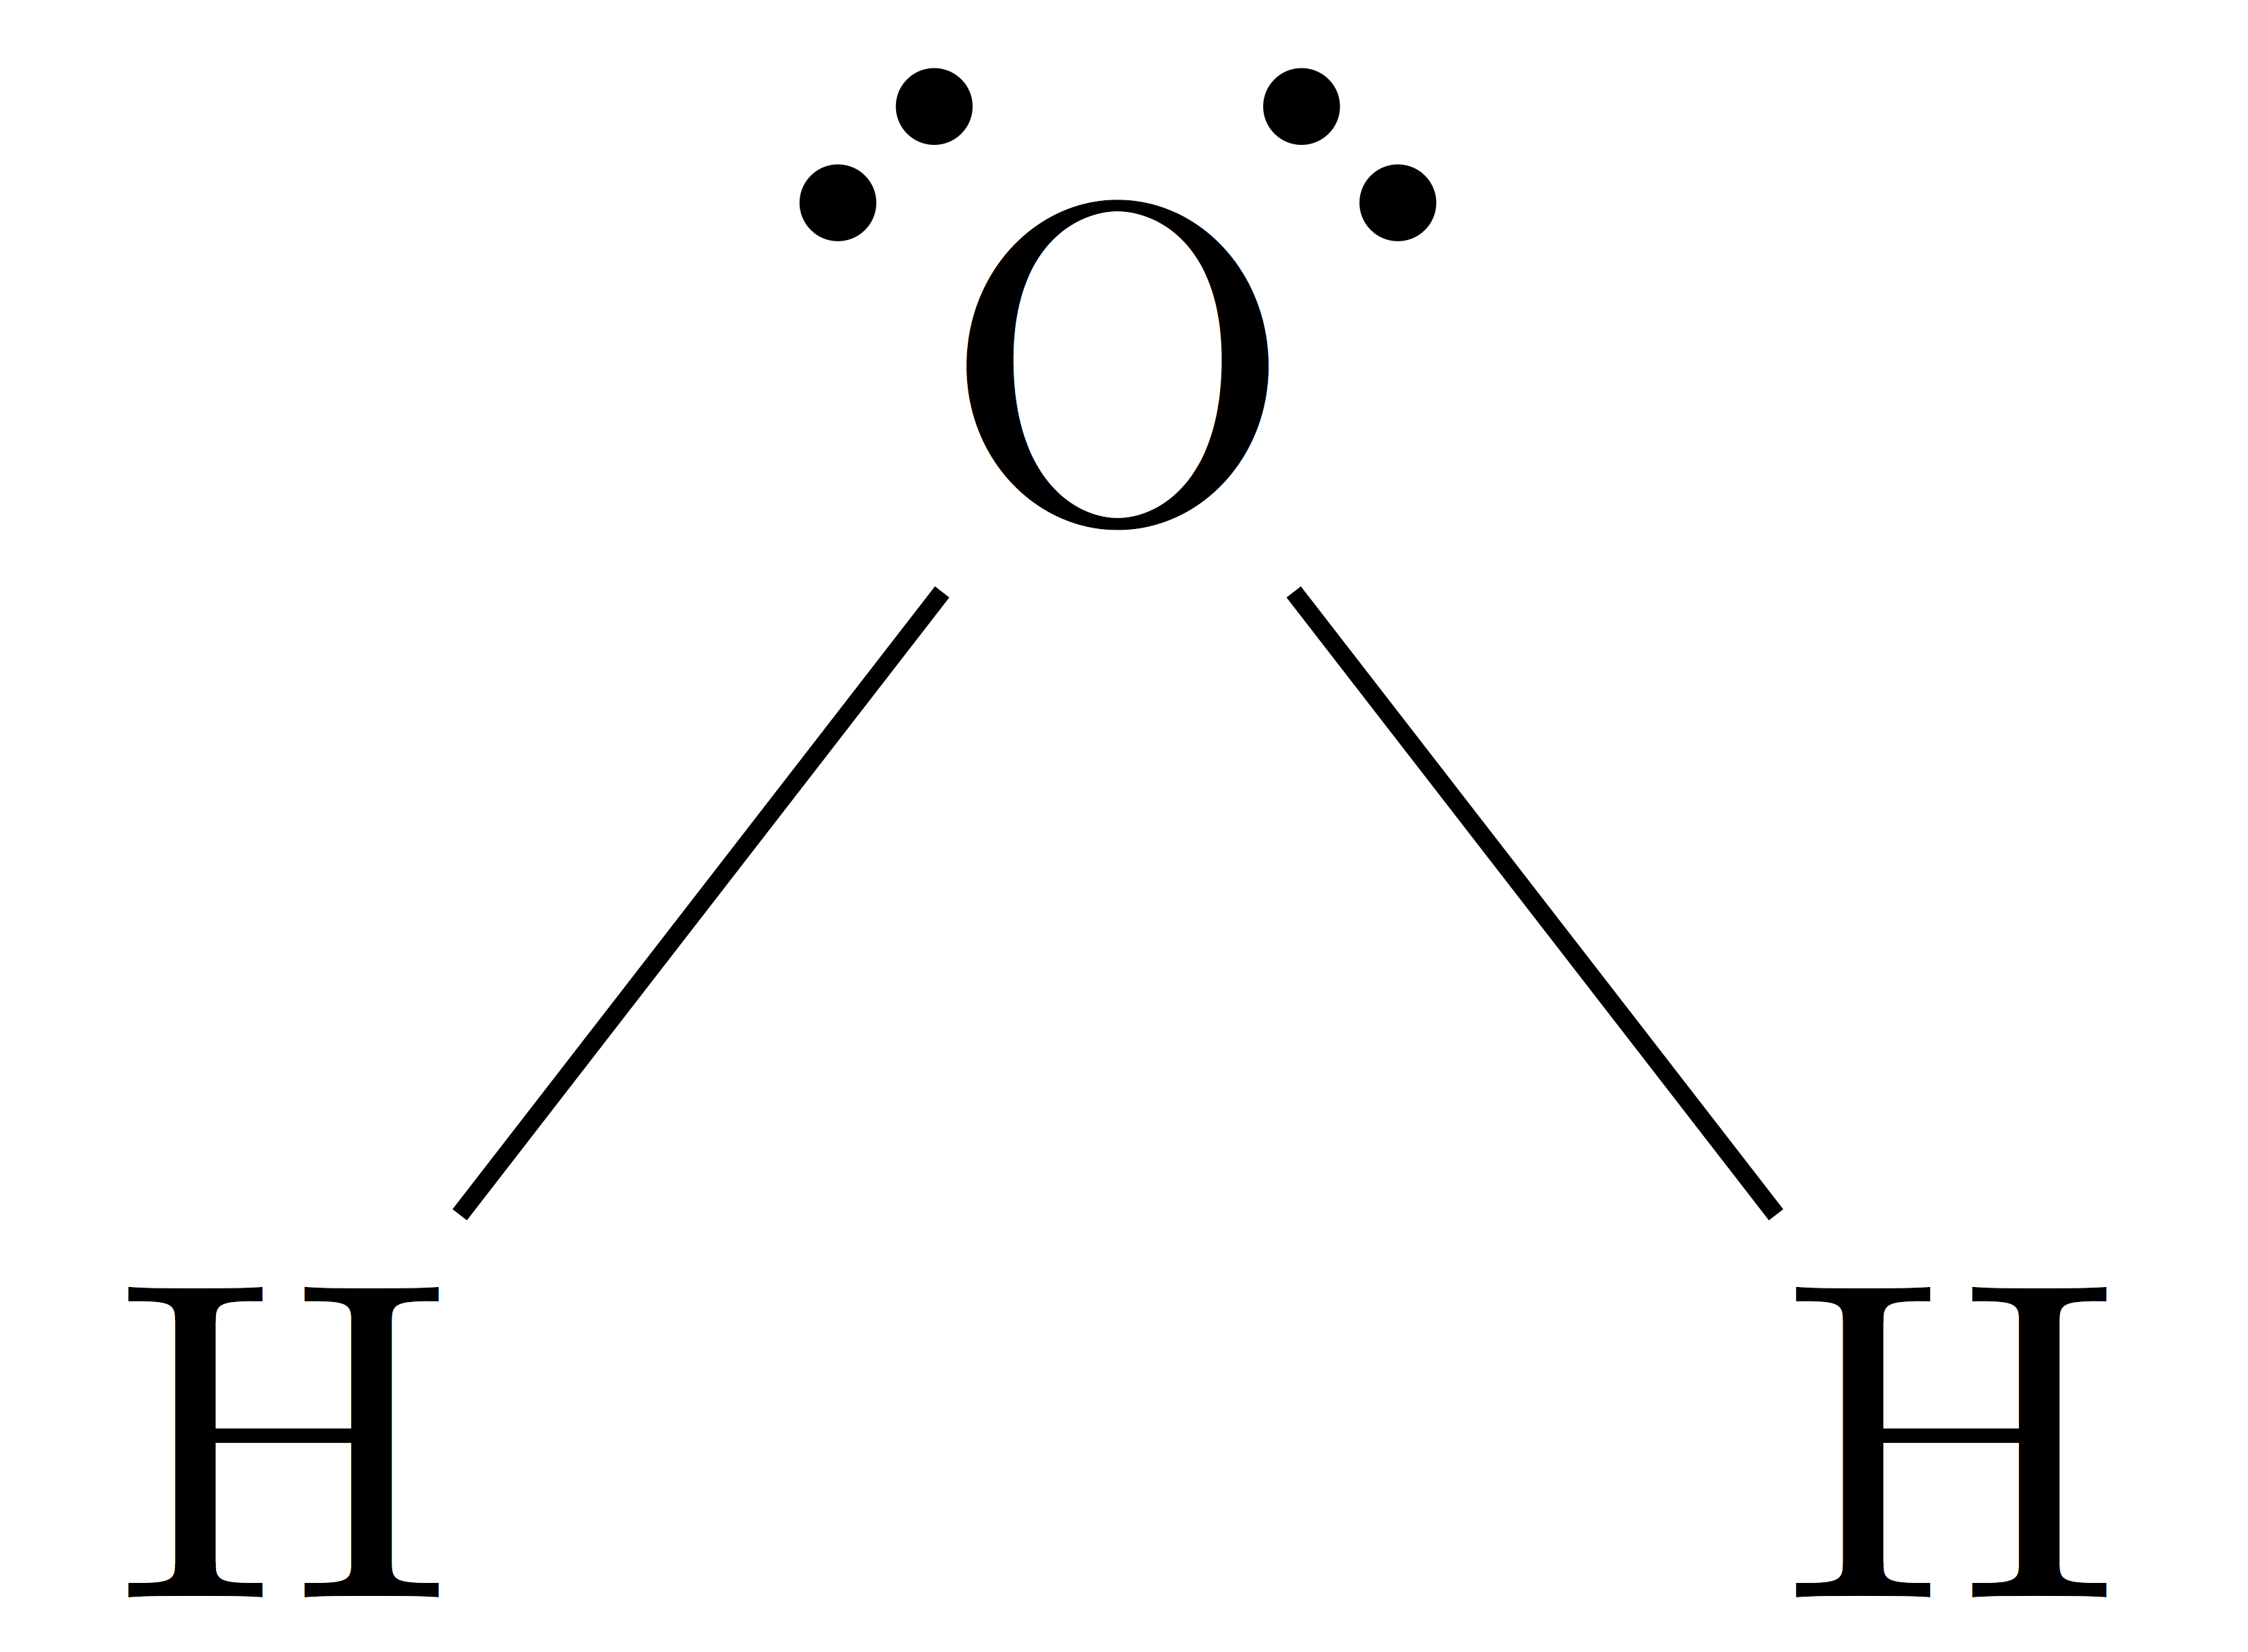
\includegraphics[width=83px]{/Users/shauryasingh/Documents/notes/class/orgs/chem/images/H2O.png}
\end{center}
The lewis structure for \(\ce{NH3}\) is
\begin{align}
\chemfig{\charge{90=\:}{N}(-{H})(-[:-90]{H})(-[:-180]{H})}
\end{align}
The lewis structure for \(\ce{HCl}\) is
\begin{align}
\chemfig{{H}(-\charge{90=\:, 0:2pt=\:, -90=\:}{Cl})}
\end{align}
The lewis structure for \(\ce{CCl4}\) is
\begin{align}
\chemfig{{C}(-\charge{90=\:, 0:2pt=\:, -90=\:}{Cl})(-[:-90]\charge{0:2pt=\:, -90=\:, -180:2pt=\:}{Cl})(-[:-180]\charge{90=\:, -180:2pt=\:, -90=\:}{Cl})(-[:-270]\charge{90=\:, 180:2pt=\:, 0=\:}{Cl})}
\end{align}

\subsection{Give the VSEPR geometry for each for each of the molecules listed in \#14.}
\label{sec:orga96a92f}
\begin{enumerate}
\item \(\ce{C2H2}\) has a linear VSEPR geometry
\item \(\ce{H2O}\) has a bent VSEPR geometry
\item \(\ce{NH3}\) has a trigonal pyramidal VSEPR geometry
\item \(\ce{HCl}\) has a linear VSEPR geometry
\item \(\ce{CCl4}\) has a tetrahedral VSEPR geometry
\end{enumerate}

\subsection{Tell whether each of the molecules listed in \#14 is polar or nonpolar.}
\label{sec:org3adbc12}
\begin{enumerate}
\item \(\ce{C2H2}\) is nonpolar
\item \(\ce{H2O}\) is polar
\item \(\ce{NH3}\) is polar
\item \(\ce{HCl}\) is polar
\item \(\ce{CCl4}\) is nonpolar
\end{enumerate}

\subsection{What primary type of intermolecular force (IMFs) would attract the molecules in \#14. Which molecules would have the highest boiling points? The lowest? (Just estimate based on what you know.)}
\label{sec:orgc05e1be}
\begin{enumerate}
\item \textbf{The primary types of intermolecular forces (IMFs) that would attract the molecules in \#14 are}
\begin{enumerate}
\item \(\ce{C2H2}\) primarily has London dispersion forces
\item \(\ce{H2O}\) primarily has hydrogen bonds, a type of dipole-dipole force
\item \(\ce{NH3}\) primarily has hydrogen bonds, a type of dipole-dipole force
\item \(\ce{HCl}\) primarily has dipole-dipole forces
\item \(\ce{CCl4}\) primarily has London dispersion forces
\end{enumerate}
\item \textbf{The molecules that have the highest boiling points and lowest boiling points are}
\begin{enumerate}
\item \(\ce{H2O}\) and \(\ce{NH3}\)  have the highest boiling points, since they have hydrogen bonds
\item \(\ce{C2H2}\) and \(\ce{CCl4}\) have the lowest boiling points, since they have London dispersion forces
\end{enumerate}
\end{enumerate}

\subsection{Name each of the following compounds:}
\label{sec:org450820d}
\begin{enumerate}
\item \(\ce{P4O6}\) is named as Tetraphosphorus hexoxide
\item \(\ce{KOH}\) is named as Potassium hydroxide
\item \(\ce{N2}\) is named as Nitrogen
\item \(\ce{PH3}\) is named as Phosphorus trihydride
\item \(\ce{BF3}\) is named as Boron trifluoride
\item \(\ce{AgCl}\) is named as Silver chloride
\item \(\ce{KHCO3}\) is named as Potassium bicarbonate
\item \(\ce{AgNO3}\) is named as Silver nitrate
\end{enumerate}

\subsection{Write formulas for each of the following compounds:}
\label{sec:org3a5d347}
\begin{enumerate}
\item The formula for sodium cyanide is \(\ce{NaCN}\)
\item The formula for tin(II) fluoride is \(\ce{SnF2}\)
\item The formula for lead(II) nitrate is \(\ce{Pb(NO3)2}\)
\item The formula for iron(III) oxide is \(\ce{Fe2O3}\)
\item The formula for calcium phosphate is \(\ce{Ca3(PO4)2}\)
\item The formula for sodium bromate is \(\ce{NaBrO3}\)
\item The formula for hydrogen iodide is \(\ce{HI}\)
\item The formula for sodium sulfate is \(\ce{Na2SO4}\)
\item The formula for manganese dioxide is \(\ce{MnO2}\)
\item The formula for potassium chlorate is \(\ce{KClO3}\)
\item The formula for potassium hypochlorite is \(\ce{KClO}\)
\item The formula for lithium hydride is \(\ce{LiH}\)
\item The formula for barium chloride is \(\ce{BaCl2}\)
\item The formula for magnesium oxide is \(\ce{MgO}\)
\item The formula for copper(I) oxide is \(\ce{Cu2O}\)
\end{enumerate}

\subsection{Give the names of the following acids}
\label{sec:orgba4758f}
\begin{enumerate}
\item \(\ce{H2SO3}\) is named as Sulfurous acid
\item \(\ce{HI}\) is named as Hydroiodic acid
\item \(\ce{HBr}\) is named as Hydrobromic acid
\item \(\ce{HNO2}\) is named as Nitrous acid
\item \(\ce{H3PO4}\) is named as Phosphoric Acid
\item \(\ce{HCl}\) is named as Hydrochloric acid
\end{enumerate}

\subsection{Give formulas for the following acids:}
\label{sec:org882d10d}
\begin{enumerate}
\item Nitric acid has a formula of \(\ce{HNO3}\)
\item hydrofluoric acid has a formula of \(\ce{HF}\)
\item sulfuric acid has a formula of \(\ce{H2SO4}\)
\item hydrocyanic acid has a formula of \(\ce{HCN}\)
\item acetic acid has a formula of \(\ce{CH3COOH}\)
\end{enumerate}

\subsection{Give the names and formulas of the seven diatomic elements.}
\label{sec:org8bd2728}
\begin{enumerate}
\item \(\ce{H2}\), or Hydrogen
\item \(\ce{N2}\), or Nitrogen
\item \(\ce{O2}\), or Oxygen
\item \(\ce{F2}\), or Fluorine
\item \(\ce{Cl2}\), or Chlorine
\item \(\ce{Br2}\), or Bromine
\item \(\ce{I2}\), or Iodine
\end{enumerate}

\subsection{Solve the following problems involving scientific notation without a calculator.}
\label{sec:org5f538c1}
\begin{enumerate}
\item The solution is \(8*10^7\)
\begin{align*}
(2*10^3)(4*10^4)&=(2*4)(10^3*10^4)\\
&=8(10^3*10^4)\\
&=8*10^{^}{3+4}\\
&=8*10^7
\end{align*}
\item The solution is \(4.2*10^{}^{12}\)
\begin{align*}
(6*10^5)(7*10^6)&=(6*7)(10^5*10^6)\\
&=42(10^5*10^6)\\
&=42*10^{^}{5+6}\\
&=42*10^{11}\\
&=4.2*10^{12}
\end{align*}
\item The solution is \(1.05*10^{14}\)
\begin{align*}
(7*10^4)(5*10^6)(3*10^2)&=(7*5*3)(10^4*10^6*10^2)\\
&=105(10^4*10^6*10^2)\\
&=105*10^{^}{4+6+2}\\
&=105*10^{12}^{}^{}\\
&=1.05*10^{14}
\end{align*}
\item The solution is \(2.5*10^3\)
\begin{align*}
\frac{(2*10^7)}{(8*10^3)}&=\frac{2}{8}*\frac{10^7}{10^3}\\
&=\frac{2}{8}*\frac{10^{7-3}}{1}\\
&=0.25*10^{7-3}\\
&=0.25*10^4^{}\\
&=2.5*10^3
\end{align*}
\item The solution is \(2*10^2\)
\begin{align*}
\frac{(4*10^6)}{(2*10^4)}&=\frac{4}{2}*\frac{10^6}{10^4}\\
&=2*10^{6-4}\\
&=2*10^2
\end{align*}
\item The solution is \(5*10^{10}\)
\begin{align*}
\frac{(2*10^3)}{(4*10^{-8})}&=\frac{2}{4}*\frac{10^3}{10^{-8}}\\
&=0.5*10^{3-(-8)}\\
&=0.5*10^{3+8}\\
&=0.5*10^{11}\\
&=5*10^{10}
\end{align*}
\item The solution is \(6*10^8\)
\begin{align*}
\frac{(5*10^6)(2*10^3)(3*10^3)}{(5*10^4)}&=\frac{(5*2*3)(10^6*10^3*10^3)}{(5*10^4)}\\
&=\frac{(30)(10^{6+3+3})}{(5*10^4)}\\
&=\frac{(30)(10^{12})}{(5*10^4)}\\
&=\frac{(3*10^{13})}{(5*10^4)}\\
&=\frac{3}{5}*\frac{10^{13}}{10^4}\\
&=0.6*10^{13-4}\\
&=0.6*10^9\\
&=6*10^8
\end{align*}
\item The solution is \(5*10^3^{}\)
\begin{align*}
\frac{(4*10^6)(5*10^{-3})}{(8*10^{-4})(5*10^3)}&=\frac{(4*5)(10^6*10^{-3})}{(8*5)(10^{-4}*10^3)}\\
&=\frac{(20)(10^{6-3}^{})}{(40)(10^{-4+3})}\\
&=\frac{(20)(10^3)}{(40)(10^{-1})}^{}\\
&=\frac{(2)(10^4)}{(4)(10^0)}^{}\\
&=\frac{2}{4}*\frac{10^4}{10^0}\\
&=0.5*10^4\\
&=5*10^3
\end{align*}
\end{enumerate}

\subsection{The structures and normal boiling points of dimethyl ether and ethanol are given in the table above.}
\label{sec:orgc9f9aff}
\begin{enumerate}
\item \textbf{Which of the following diagrams best helps to explain the difference in boiling point of the two compounds?}

The answer is \textbf{B}, since it best shows the difference between hydrogen bonds.

\item \textbf{Describe your reasoning for selecting the answer you did and specifically identify the type of intermolecular forces represented.}

Dimethyl either consists of dipole-dipole interactions or dispersion forces, whereas Ethanol consists of hydrogen bonds, and diagram B best highlights that.
\end{enumerate}

\subsection{Shown below are three models that can be used to represent a molecule of ammonia. Select one of the models. Each model has its pros and cons.}
\label{sec:org892926a}
I chose to compare the benefits and drawbacks of the \textbf{lewis structure} model.
\begin{enumerate}
\item \textbf{One aspect of the ammonia molecule that the model represents accurately/well}

The Lewis structure model allows the reader to easily see where all the electrons are, as well as if each atom obeys the octet rule. You can also which electrons are bonding, as well as which electrons are non-bonding and lone pairs.

\item \textbf{One aspect of the ammonia molecule that the model does not represent accurately/well.}

It is difficult to show resonance structures with a lewis structure. There is also a lack of 3 dimensional modeling with the lewis structure. Lewis structures only imply shape, in order to find the 3 dimensional shape of a molecule, you have to use other knowledge, using VSEPR.
\end{enumerate}
\end{document}
